\documentclass[titlepage=firstiscover, captions=tableheading]{scrartcl}

\usepackage{polyglossia}
\setmainlanguage{german}

\usepackage{fontspec}
\usepackage{amsmath}
\usepackage{amssymb}
\usepackage{mathtools}
\usepackage[locale=DE, separate-uncertainty=true, per-mode=symbol-or-fraction]{siunitx}
\usepackage{microtype}
\usepackage{xfrac}
%\usepackage{subcaption}
%\usepackage{graphicx}
%\usepackage{grffile}
\usepackage{booktabs}
\usepackage{biblatex}
\addbibresource{lit.bib}



\usepackage[math-style=ISO,bold-style=ISO,sans-style=italic,nabla=upright,partial=upright,]{unicode-math}
\setmathfont{Latin Modern Math}
\setlength{\parindent}{0em}

\begin{document}
\setlength{\parindent}{0em}

%\pagestyle{empty}
%Keine Seitenzahl

%
\title{US2 Scanverfahren in der Ultraschalltechnik}
\author{Katharina Brägelmann \and Tobias Janßen \and katharina.braegelmann@tu-dortmund.de \and tobias2.janssen@tu-dortmund.de}
\date{Durchführung: 29. Mai 2018, Abgabe: 5. Mai 2018}
\maketitle

\tableofcontents

%\input{lit.bib}
\pagenumbering{arabic}

\tableofcontents
\newpage

\section{Zielsetzung}
\input{Zielsetzung.txt}


\section{Theorie}
%Licht allgemein
Licht lässt sich sowohl als Teilchen als auch als Welle auffassen.
Bei Prozessen, bei denen es auf das einzelne Lichtquant ankommt, ist eine Beschreibung als Welle nicht sinnvoll, so zum Beispiel bei dem Photoeffekt oder bei dem Comptoneffekt.
Prozesse, bei denen über große Anzahlen von Lichtquanten gemittelt werden kann, lassen sich durch eine Wellendarstellung beschreiben.
%Interferenz
\\Lichtwellen können dem Prinzip der Interferenz unterliegen.
Dabei überlagern sich mindestens zwei Lichtwellen.
Liegen zwei Wellenberge zweier Wellen mit gleicher Wellenlänge übereinander, addieren sie sich zu einem größeren Maximum.
Zwei Wellentäler addieren sich zu einem tieferen Wellental.
Diese beiden Phänomene fallen unter die konstruktive Interferenz.
Ein Wellenberg, der auf einem Wellental liegt, löschen sich Wellenberg und Wellental aus.
Dies wird destruktive Interferenz genannt.
Sind die Wellenlängen der beiden interferierenden Wellen nicht gleich, kommt es zu sogenannten Schwebungen und Wellenpakteten.
In diesem Versuch wird nur die Interferenz zweier gleicher Wellen betrachtet.
%Huygens
\\Das Huygens'sche Prinzip .
Es sagt aus, dass jeder Oszillator einer Welle der Ausgangspunkt einer neuen Elementarwelle sein kann.
Die einzelnen Elementarwellen summieren sich zu einer neuen Wellenfront.
Es kommt zur Interferenz der Elementarwellen.
Bei einer Grenzfläche, einem Einzelspalt oder einem Doppelspalt zeigt sich dieses Phänomen.
%Einzelspalt
\\Zunächst wird der Einzelspalt behandelt.
Dabei gibt es zwei Varianten die Beugung am Einzelspalt zu untersuchen; einerseits gibt es die Fresnel'sche Beugung, andererseits die Fraunhofer'sche Beugung (Abb. \ref{fig:fresnelfraunhofer}).
\begin{figure}[h!]
  \centering
  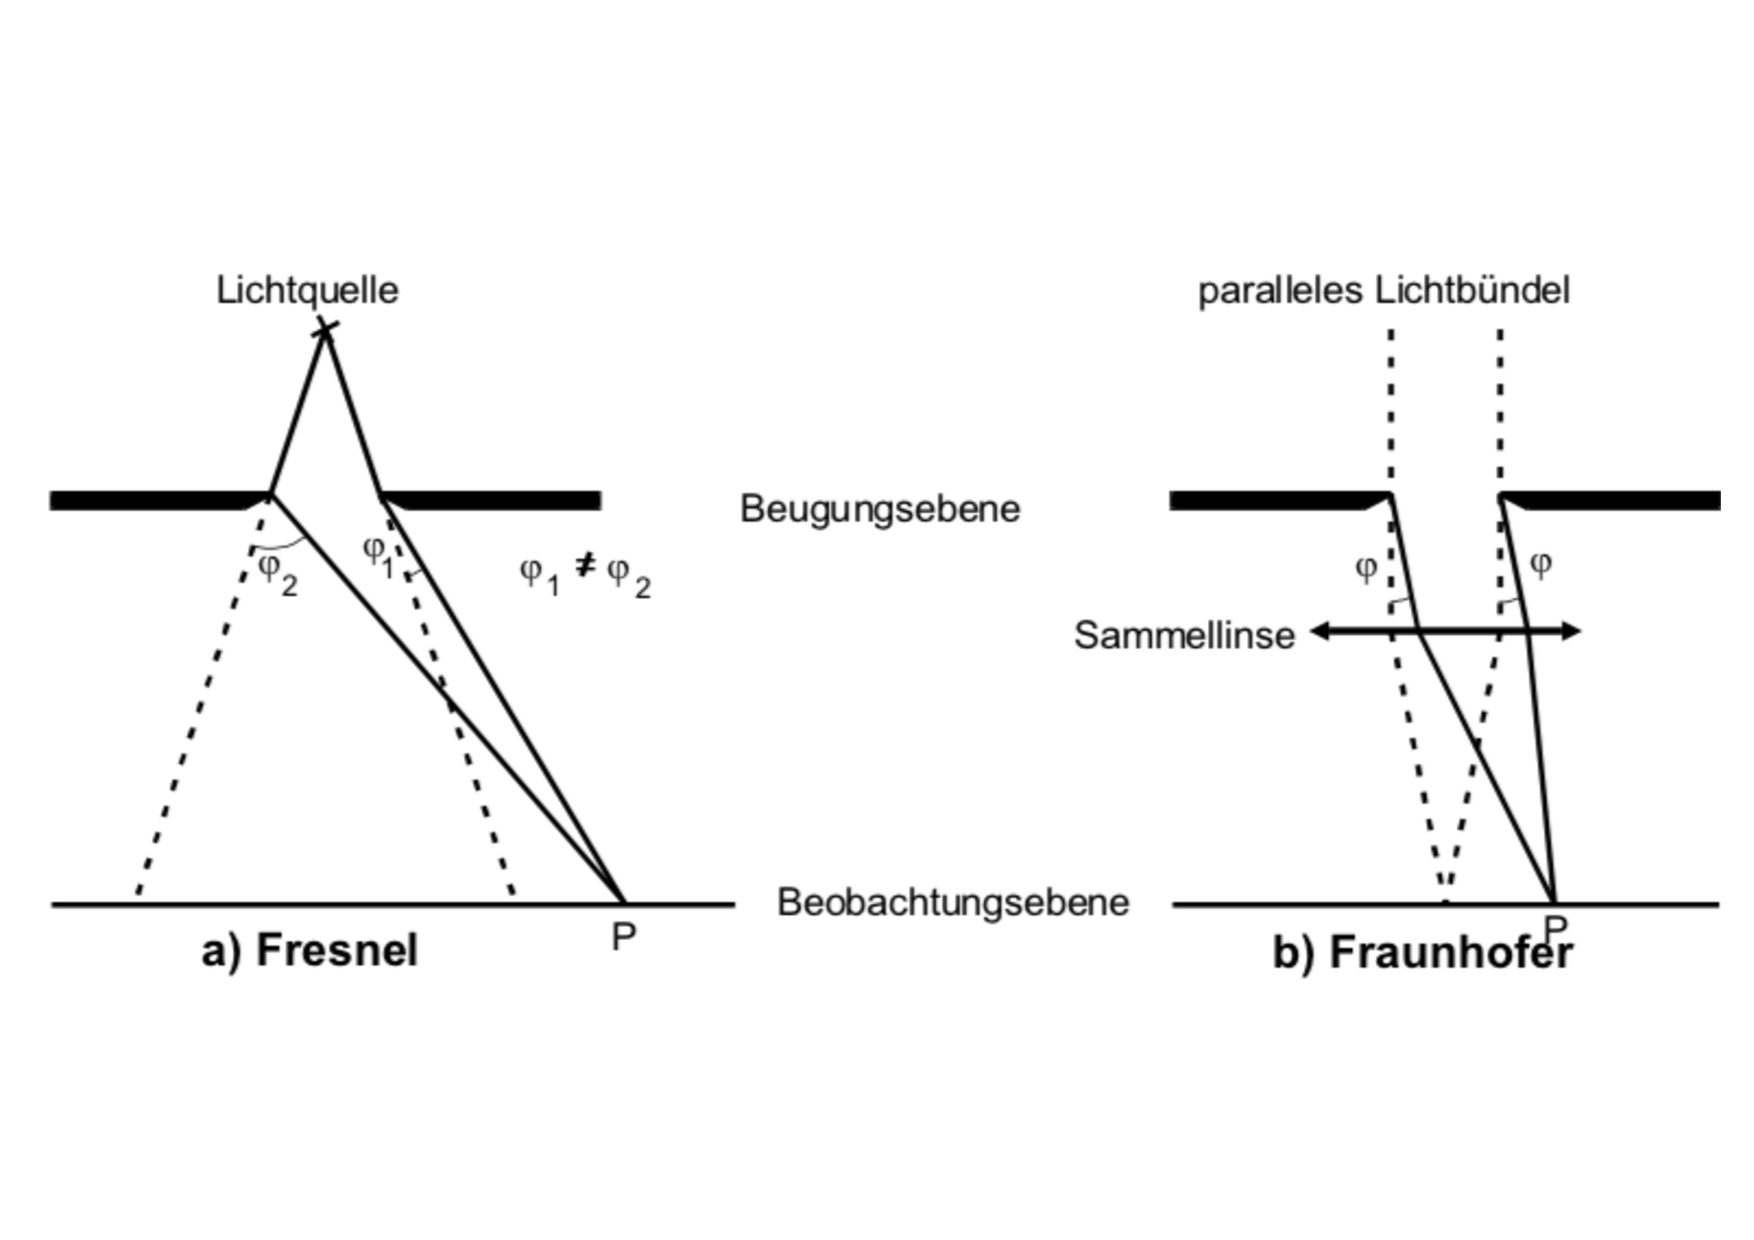
\includegraphics[width=\textwidth]{fresnelfraunhofer.pdf}
  \caption{Fresnel'sche und Fraunhofer'sche Beugung \cite{1}}
  \label{fig:fresnelfraunhofer}
\end{figure}
Bei der Fresnel'schen Beugung sind die Lichtquelle und die Bildebene nah an dem Spalt.
Die Fraunhofer'sche Beugung funktioniert mit größeren Abständen:
Die Lichtquelle ist so weit weg von dem Spalt, dass die einfallenden Lichtstrahlen parallel sind.
Auch die Bildebene ist weiter weg von dem Spalt.
In diesem Versuch wird die Fraunhofer'sche Beugung verwendet.
Der Strahlengang am Einzelspalt ist in Abbildung \ref{fig:einzelspalt} dargestellt.
\begin{figure}[h!]
  \centering
  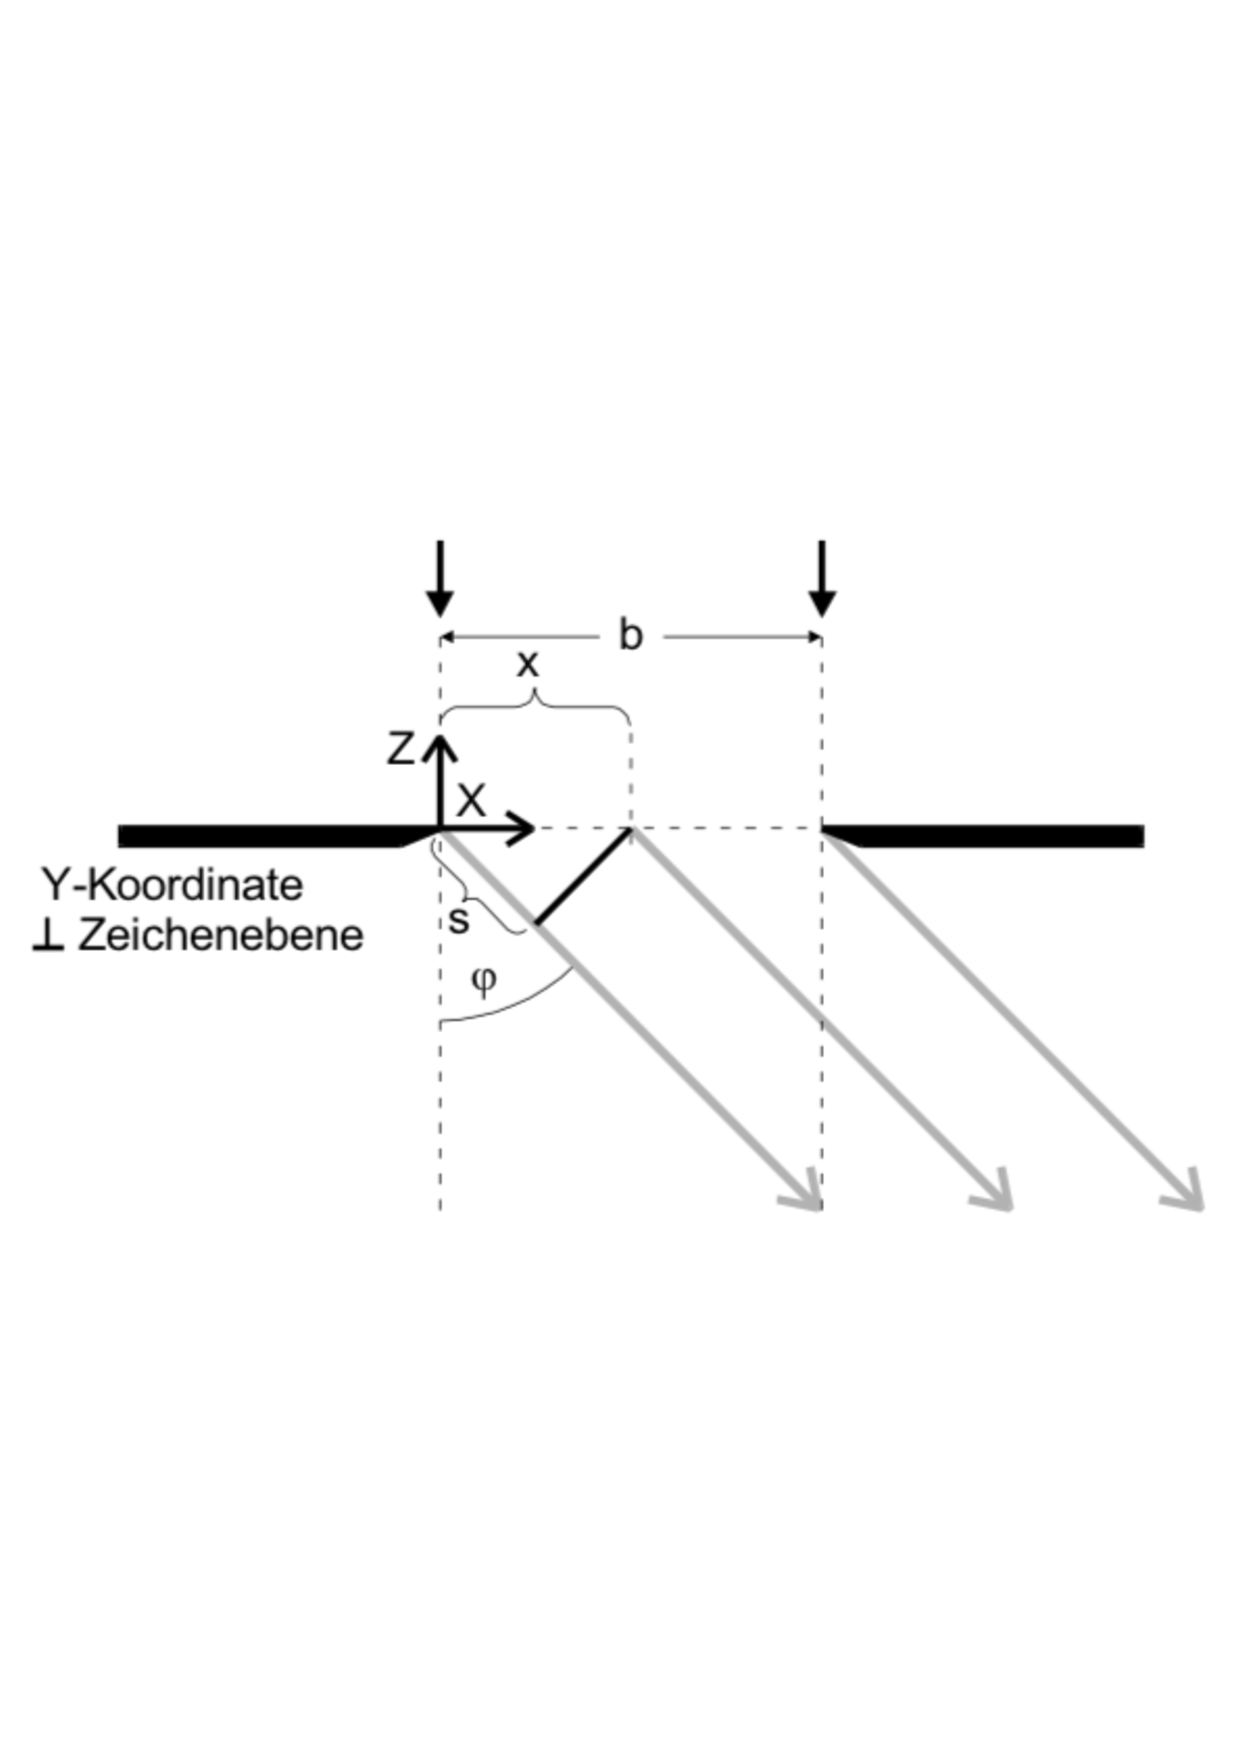
\includegraphics[width=\textwidth]{einzelspalt.pdf}
  \caption{Huygens'sches Prinzip am Einzelspalt \cite{1}}
  \label{fig:einzelspalt}
\end{figure}
Dabei ist zu erkennen, dass bei einer Beugung um den Winkel $\varphi$ ein Gangunterschied zwischen den Strahlen entsteht.
Eine Lichtwelle kann hier die Form
\begin{align*}
  A(z, t) = A_{0} \exp{ \left[i \left( \omega t - \frac{2 \pi z}{\lambda} \right) \right]}
\end{align*}
Die entstehende Phasendifferenz beim Gangunterschied $s$ zwischen zwei Strahlen der Wellenlänge $\lambda$ beträgt dann:
\begin{align*}
  \delta = \frac{2 \pi s}{\lambda} = \frac{2 \pi x \sin{(\varphi)}}{\lambda}
\end{align*}
An den Spalten wird die Welle also bei den interferierenden Wellenlängen um den Winkel $\varphi$ gebeugt.
Die Amplitude lässt sich am Einzelspalt durch das Integral über die Spaltbreite $b$ berechnen:
\begin{align*}
  B(z, t, \varphi) = A_{0} \int_{0}^{b} \exp{ \left[i \left(\omega t - \frac{2 \pi z}{\lambda} + \delta \right) \right]} dx.
\end{align*}
Mit einigen Umformungen wird daraus:
\begin{align*}
  B(z, t, \varphi) = A_{0} \exp{ \left[ i \left(\omega t - \frac{2 \pi z}{\lambda} \right) \right]}
  \exp{\left[  i \frac{\pi b \sin{(\varphi)}}{\lambda} \right]}
  \frac{\lambda}{\pi \sin{(\varphi)}} \sin{ \left( \frac{\pi b \sin{(\varphi)}}{\lambda} \right)}.
\end{align*}
Die beiden exponentiellen Faktoren sind für die Rechnung unerheblich.
Damit lässt sich $B(z, t, \varphi)$ zu folgender Gleichung überführen:
\begin{align*}
    B(\varphi)= A_{0} b \sin{\left( \frac{\pi b \sin{(\varphi)}}{\lambda} \right)} \frac{\lambda}{\pi b \sin{(\varphi)}}.
\end{align*}
Die Intensität ist proportional zum Betragsquadrat der Amplitude $B(\varphi)$:
\begin{align}
  I(\varphi) \propto B^2(\varphi) = A_{0}^2 b^2 \sin^2{\left( \frac{\pi b \sin{(\varphi)}}{\lambda} \right)} \frac{\lambda^2}{\pi^2 b^2 \sin^2{(\varphi)}}
  \label{eqn:einzelspalt}
\end{align}
Die Intensitätsminima liegen bei
\begin{align*}
  \varphi(k) = \arcsin{\left( \pm \frac{n \lambda}{b} \right)}.
\end{align*}
%Doppelspalt
\\Der Doppelspalt verhält sich wie die Überlagerung zweier Einzelspalte (Abb. \ref{fig:doppelspalt}), bei der durch die Interferenz ein zusätzlicher Cosinusterm hinzukommt (Gleichung \eqref{eqn:doppelspalt}).
\begin{figure}[h!]
  \centering
  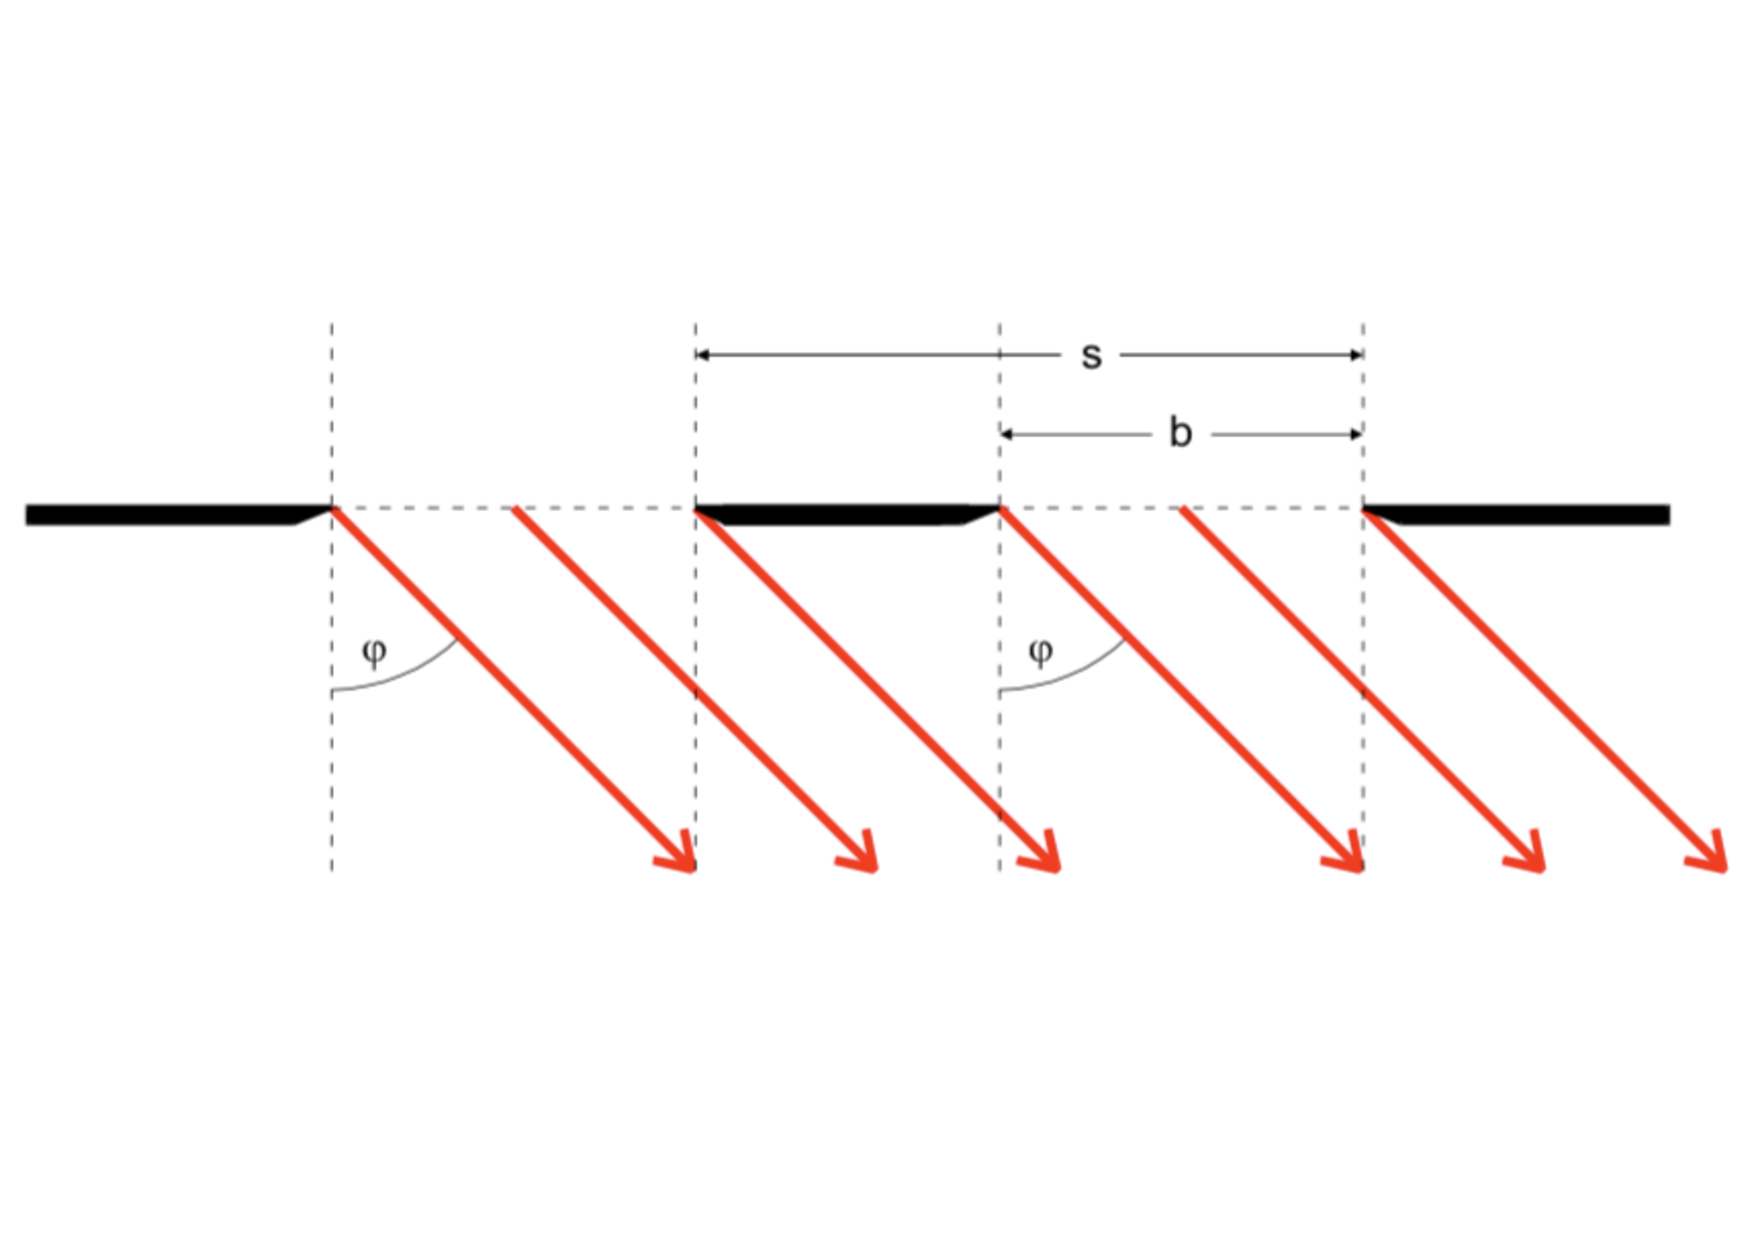
\includegraphics[width=\textwidth]{doppelspalt.pdf}
  \caption{Strahlengang am Doppelspalt \cite{1}}
  \label{fig:doppelspalt}
\end{figure}
Die Intensität eines Spalts des Abstands $b$ verhält sich dann wie folgt:
\begin{align}
  I(\varphi) \propto B^2(\varphi)= 4 \cos^2{ \left( \frac{\pi s \sin{(\varphi)}}{\lambda} \right)} \left( \frac{\lambda}{\pi b \sin{(\varphi)}} \right)^2 \sin^2{\left( \frac{\pi b \sin{(\varphi)}}{\lambda} \right)}.
  \label{eqn:doppelspalt}
\end{align}
Die Intensitätsminima liegen bei
\begin{align*}
  \varphi_{1}(n) &=& \arcsin{\left( \pm \frac{n \lambda}{b} \right)},  &&  n=(1, 2, 3, 4, ...)\\
  \varphi_{2}(k) &=& \arcsin{ \left( \frac{2k+1}{2s} \right)}       ,  &&  k=(0, 1, 2, 3, 4, ...).\\
\end{align*}
%fouriertransformation
\\Mit einer Fouriertransformation lässt sich die Amplitudenverteilung bei der Fraunhofer'schen Beugung allgemeiner beschreiben.
Die Fouriertransformierte hat die Form
\begin{align*}
  g(\zeta)= \int_{-\infty}^{\infty} f(x) \exp{(ix \zeta)} dx = A_{0} \int_{0}^{b} \exp{(ix \zeta)} dx = \frac{A_{0}}{i \zeta}(-1 \exp{(ib\zeta)}).
\end{align*}
Daraus ergibt sich
\begin{align*}
   \zeta = \frac{2 \pi \sin{(\varphi)}}{\lambda}.
\end{align*}
Die Fouriertransformation beschreibt also das Huygens'sche Prinzip mathematisch.

\FloatBarrier



\section{Aufbau und Durchführung}
Auf einer zweifach eingespannten, drehbaren Achse können verschiedene Körper befestigt werden.
Die Achse ist über eine Feder mit dem Rahmen verbunden.
Zur Berechnung späterer Trägheitsmomente werden die Konstanten der Feder benötigt.
\\D wird bestimmt, indem eine Federwaage an einem bestimmten Abstand zur Achse an eine nahezu masselosen Stange ansetzt wird und diese Stange den Winkel $\phi$ ausgelenkt wird.
An der Federwaage ist die zugehörige Kraft ablesbar.
Es wird die Kraft für 10 Winkel gemessen.
\\Das Eigenträgheitsmoment $I_D$ wird bestimmt, indem eine Stange mit zwei zylinderförmigen Gewichten senkrecht zur Drillachse befestigt wird und diese in Schwingung versetzt wird.
Die Schwingungsdauer ist für 10 unterschiedliche Abstände der Massen zur Drehachse zu messen.
\\Anschließend wird das Trägheitsmoment von einem liegenden und einem stehenden Zylinder ermittelt.
Dafür wird wieder die Schwingungsdauer der Körper gemessen.
\\Eine Holzpuppe wird nach der Vermessung ihrer Proportionen und nach Messen des Gewichtes, auf die Drillachse gesteckt.
Es werden für zwei verschiedenen Körperhaltungen die Schwingungszeiten ermittelt.
Zunächst werden die Schwingungsdauern der Puppe mit angelegten Armen gemessen, dann werden die Schwingungsdauern der selben Puppe mit seitlich ausgestreckten Armen gemessen.

\newpage

\section{Auswertung}
Die Photodiode hat von dem Spalt den Abstand
\begin{align*}
  L=\SI{0,9}{m}.
\end{align*}
Der Laser leuchtet mit einer Wellenlänge von
\begin{align*}
  \lambda=\SI{635e-9}{nm}.
\end{align*}
Die Messung des Dunkelstroms ergibt:
\begin{align*}
  I_{\text{du}}=\SI{0,58}{nA}.
\end{align*}
Bei allen nachfolgenden Intensitäten wird der Dunkelstrom $I_{du}$ abgezogen um den realen Wert zu erhalten.
Die maximale Intensität jeder Messung wird als Nullpunkt genommen.
\subsection{Einzelspalt 1}
Die Spaltbreite ist gegeben als:
\begin{align*}
  b=\SI{0,022e-3}{m}.
\end{align*}
Die gemessenen Werte sind in der Tabelle \ref{tab:1a} und in der Abbildung \ref{fig:1a} dargestellt.\\
Mit Phython wird eine Ausgleichsrechnung nach der Form der Gleichung \ref{eqn:einzelspalt} bestimmt.
Die durch Python errechnete Spaltbreite beträgt:
\begin{align*}
  b=\SI{0,045\pm0,001e-3}{m}.
\end{align*}
\begin{table}[h!]
  \centering
  \caption{Messwerte für den Einzelspallt mit $b=\SI{0,022e-3}{m}$}
  \label{tab:1a}
  \begin{tabular}{c c c c}
    \toprule
       Auslenkung /mm  & Intensität /nA & Auslenkung /mm& Intensität /nA  \\
    \midrule

	  0,00	  	& 7,92 & -23,94	  	& 0,52\\
	 -0,14	  	& 7,92 & -24,44	    &	0,52\\
	 -1,44	  	& 7,72 & -24,94	    &	0,50\\
	 -1,94	  	& 7,42 & -25,44	    &	0,50\\
	 -2,44	  	& 7,02 & -25,94	  	& 0,43\\
	 -2,94	  	& 6,62 & -26,44	  	& 0,42\\
	 -3,44	  	& 6,12 & -26,94	  	& 0,42\\
	 -3,94	  	& 5,62 & 0,06	    	& 8,62\\
	 -4,44	  	& 5,02 & 0,56	    	& 8,42\\
	 -4,94	  	& 4,42 & 1,06	    	& 8,12\\
	 -5,44	  	& 3,82 & 1,56	    	& 7,82\\
	 -5,94	  	& 3,32 & 2,06	    	& 7,22\\
	 -6,44	  	& 2,82 & 3,06	    	& 6,22\\
	 -6,94	  	& 2,32 & 4,06	    	& 6,22\\
	 -7,44	  	& 1,92 & 5,06	    	& 5,12\\
	 -7,94	  	& 1,62 & 6,06	    	& 4,02\\
	 -8,44	  	& 1,32 & 7,06	    	& 2,22\\
	 -8,94	  	& 1,12 & 8,06	    	& 1,62\\
	 -9,44	  	& 0,92 & 8,56	    	& 1,27\\
	 -9,94	  	& 0,80 & 9,06	    	& 1,12\\
	 -10,44	  	& 0,72 & 9,56	    	& 0,97\\
	 -10,94	  	& 0,72 & 10,06    	& 0,87\\
	 -11,44	  	& 0,72 & 10,56	  	& 0,82\\
	 -11,94	  	& 0,72 & 11,06	  	& 0,77\\
	 -12,44	  	& 0,75 & 11,56	  	& 0,72\\
	 -12,94	  	& 0,75 & 12,06	  	& 0,72\\
	 -13,44	  	& 0,77 & 12,56	  	& 0,68\\
	 -13,94	  	& 0,77 & 13,06	  	& 0,68\\
	 -14,44	  	& 0,77 & 13,56	  	& 0,67\\
	 -14,94	  	& 0,77 & 14,06	  	& 0,67\\
	 -15,44	  	& 0,72 & 14,56	  	& 0,62\\
	 -15,94	  	& 0,67 & 15,06	  	& 0,62\\
	 -16,44	  	& 0,62 & 15,56	  	& 0,57\\
	 -16,94	  	& 0,57 & 16,06	  	& 0,52\\
	 -17,44	  	& 0,52 & 16,56	  	& 0,47\\
	 -17,94	  	& 0,47 & 17,06	  	& 0,42\\
	 -18,44	  	& 0,42 & 17,56	  	& 0,37\\
	 -18,94	  	& 0,42 & 18,06	  	& 0,32\\
	 -19,44	  	& 0,37 & 18,56	  	& 0,27\\
	 -19,94	  	& 0,37 & 19,06	  	& 0,27\\
	 -20,44	  	& 0,42 & 19,56	  	& 0,22\\
	 -20,94	  	& 0,42 & 20,56	  	& 0,17\\
	 -21,44	  	& 0,42 & 21,56	  	& 0,17\\
	 -21,94	  	& 0,42 & 22,56	  	& 0,17\\
	 -22,44	  	& 0,47 & 23,56	  	& 0,17\\
	 -22,94	    &	0,47 & 24,56	  	& 0,17\\
	 -23,44	  	& 0,50 & 25,56	  	& 0,17\\



\bottomrule
\end{tabular}
\end{table}

\begin{figure}
  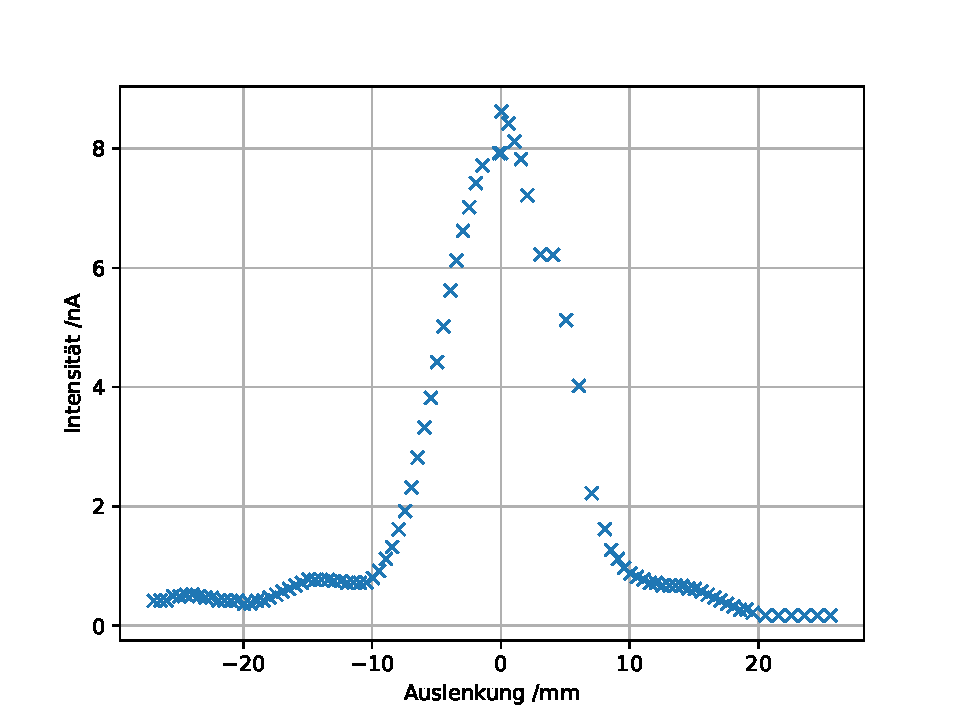
\includegraphics{1a.pdf}
  \caption{Einzelspalt 1}
  \label{fig:1a}
\end{figure}
\FloatBarrier
\subsection{Einzelspalt 2}
Die Spaltgröße ist gegeben als:
\begin{align*}
  b=\SI{0,1e-3}{m}
\end{align*}
Die gemessenen Werte sind in der Tabelle \ref{tab:1b} und in der Abbildung \ref{fig:1b} dargestellt.\\
Mit Phython wird erneut eine Ausgleichsrechnung mit Gleichung \ref{eqn:einzelspalt} ausgeführt.
Die von Python berechnete Spaltbreite beträgt:
\begin{align*}
  b = \SI{0.29\pm0.01e-3}{m}.
\end{align*}
\begin{table}[h!]
  \centering
  \caption{Messwerte für den Einzelspallt mit $b=\SI{0,1e-3}{m}$}
  \label{tab:1b}
  \begin{tabular}{c c c c}
    \toprule
       Auslenkung /mm  & Intensität /nA & Auslenkung /mm  & Intensität /nA  \\
    \midrule

    0,00		&299,42&-&-\\
   -0,50		&339,42&0,50		&179,42\\
   -1,00		&234,42&1,00		&74,42\\
   -1,50		&99,42&1,50		&44,42\\
   -2,00		&43,42&2,00		&29,42\\
   -1,31		&40,42&2,50		&24,42\\
   -2,50		&42,42&3,00		&21,92\\
   -3,00		&42,42&3,50		&19,42\\
   -3,50		&37,42&4,00		&16,92\\
   -4,00		&29,42&4,20		&16,92\\
   -4,50		&19,42&4,50		&18,42\\
   -5,00		&13,42&4,79		&18,92\\
   -5,19		&13,42&5,00		&17,92\\
   -5,50		&15,42&5,50		&14,42\\
   -6,00		&19,42&6,00		&12,92\\
   -6,50		&25,42&6,50		&13,42\\
   -7,00		&29,92&7,00		&14,92\\
   -7,13		&31,42&7,50		&15,42\\
   -7,50		&26,92&8,00		&14,92\\
   -8,00		&14,92&8,50		&10,92\\
   -8,50		&12,92&9,00		&8,42\\
   -9,00		&11,92&9,50		&6,42\\
   -9,50		&17,92&10,00		&5,82\\
   -9,73		&18,42&10,50		&4,62\\
   -10,0		&17,42&11,00		&3,92\\
   -10,5		&13,42&11,50		&3,62\\



   \bottomrule
\end{tabular}
\end{table}

\begin{figure}
  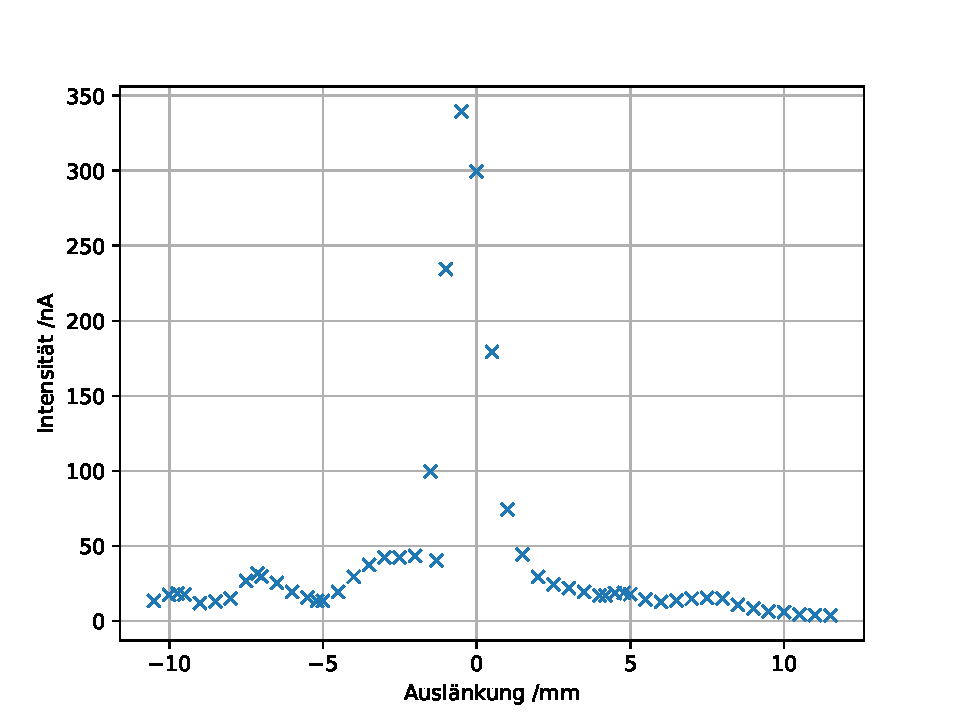
\includegraphics{1b.pdf}
  \caption{Einzelpalt 2}
  \label{fig:1b}
\end{figure}
\FloatBarrier

\subsection{Doppelspalt}
Die Spaltgrößen $b$ und der Spaltabstand $s$ sind gegeben als:
\begin{align*}
  b=\SI{0,15e-3}{m}\\
  g=\SI{0,25e-3}{m}.
\end{align*}
Die gemessenen Werte sind in der Tabelle \ref{tab:2} und in der Abbildung \ref{fig:2} dargestellt.
Die nicht-lineare Ausgleichsrechnung nach Gleichung \ref{eqn:doppelspalt} wird mit Python bestimmt.
\begin{table}[h!]
  \centering
  \caption{Messwerte für den Doppelspalt mit $b=\SI{0,15e-3}{m}$ und $g=\SI{0,25e-3}{m}$}
  \label{tab:2}
  \begin{tabular}{c c c c}
    \toprule
       Auslenkung /mm  & Intensität /nA & Auslenkung /mm  & Intensität /nA  \\
    \midrule



    0,00		& 189,42&0,00		& 179,42\\
   -0,25		& 194,42&0,25		& 134,42\\
   -0,50		& 174,92&0,50		& 79,42\\
   -0,75		& 129,92&0,75		& 45,42\\
   -1,00		& 85,42& 1,00		& 34,42\\
   -1,25		& 57,42& 1,25		& 38,42\\
   -1,50		& 52,42& 1,50		& 47,42\\
   -1,75		& 59,42& 1,73		& 51,42\\
   -2,00		& 66,42& 1,75		& 51,42\\
   -2,25		& 66,42& 2,00		& 51,42\\
   -2,50		& 61,42& 2,25		& 47,42\\
   -2,75		& 57,42& 2,50		& 47,42\\
   -3,00		& 57,42& 2,75		& 49,42\\
   -3,25		& 57,42& 3,00		& 46,42\\
   -3,50		& 52,42& 3,25		& 42,42\\
   -3,75		& 42,42& 3,50		& 30,42\\
   -4,00		& 31,42& 3,75		& 22,92\\
   -4,25		& 23,42& 4,00		& 17,92\\
   -4,50		& 21,42& 4,25		& 14,32\\
   -4,75		& 26,42& 4,35		& 13,92\\
   -5,00		& 31,42& 4,50		& 13,92\\
   -5,25		& 33,42& 4,75		& 14,42\\
   -5,50		& 30,42& 5,00		& 14,32\\
   -5,75		& 24,42& 5,25		& 13,42\\
   -6,00		& 18,42& 5,50		& 11,92\\
   -6,25		& 12,42& 5,75		& 10,92\\
   -6,50		& 9,42& 5,76		& 10,92\\
   -6,72		& 9,22& 6,00		& 11,42\\
   -6,75		& 9,32& 6,25		& 12,92\\
   -7,00		& 11,42& 6,50		& 14,42\\
   -7,25		& 14,92& 6,75		& 16,42\\
   -7,50		& 17,92& 7,00		& 16,92\\
   -7,73		& 18,42& 7,25		& 16,22\\
   -7,73		& 18,92& 7,50		& 13,92\\
   -8,00		& 17,42& 7,75		& 13,92\\
   -8,25		& 15,42& 8,00		& 9,22\\
   -8,50		& 12,92& 8,15		& 8,62\\
   -8,75		& 11,92& 8,25		& 8,42\\
   -9,00		& 11,97& 8,50		& 9,02\\
   -9,25		& 12,92& 8,75		& 9,92\\
   -9,50		& 14,42& 9,00		& 10,92\\
   -9,75		& 9,92& 9,25		& 10,42\\
   -10,00		& 9,92& 9,50		& 8,82\\
   -        &   - & 9,75		& 7,22\\
   -        &   - & 10,00	& 6,42\\



   \bottomrule
\end{tabular}
\end{table}

\begin{figure}
  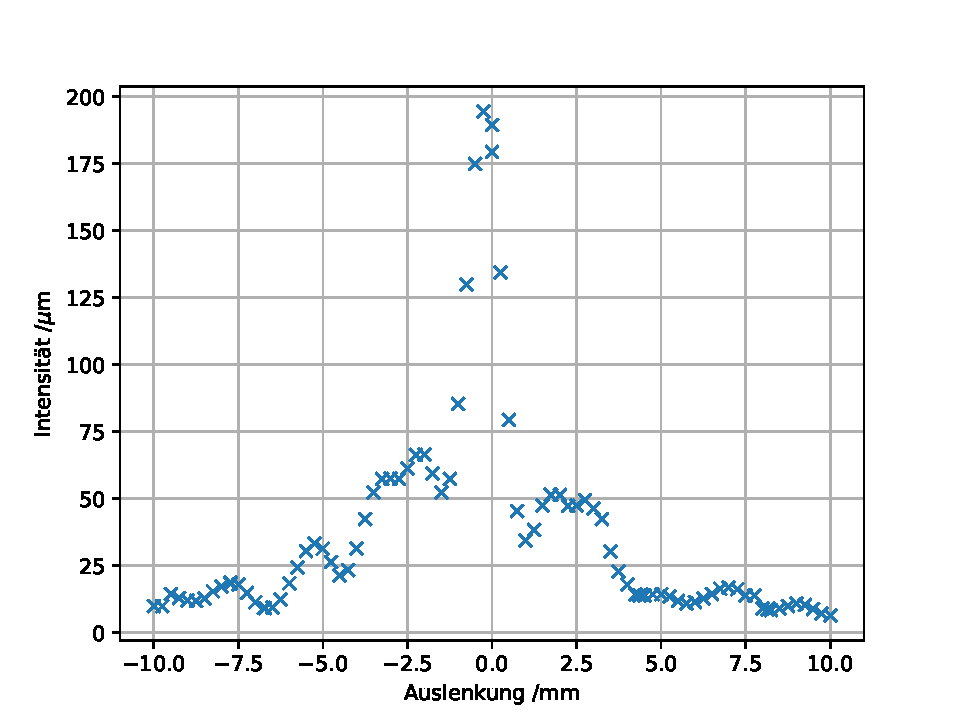
\includegraphics{2.pdf}
  \caption{Doppelspalt}
  \label{fig:2}
\end{figure}
\FloatBarrier

%\newpage

\section{Diskussion}
Im ersten Einzelspaltexperiment werden folgende Werte ermittelt:
\begin{align*}
  &\text{Theorie}&&b=\SI{0,022e-3}{m}\\
  &\text{Errechnet}&&b=\SI{0,045\pm0,001e-3}{m}\\
  &\text{Abweichung}&&\sigma = \pm\SI{104,5}{\percent}.
\end{align*}
Im zweiten Einzelspaltexperiment werden diese Werte ermittelt:
\begin{align*}
  &\text{Theorie}&&b=\SI{0,1e-3}{m}\\
  &\text{Errechnet}&&b=\SI{0.29\pm0.01e-3}{m}\\
  &\text{Abweichung}&&\sigma = \pm\SI{190}{\percent}.
\end{align*}
Beim Doppelspalt wird anhand von der Abbildung \ref{fig:2} deutlich,
dass die Formel des Doppelspaltes \ref{eqn:doppelspalt} deutlich besser zu den Messwerten passt als die
Formel zum Einzelspalt \ref{eqn:einzelspalt}.
Die Messungen des Experimentes haben große Fehlerquellen.
Es gibt Schwankungen in der Dunkelstrahlung.
Der Messaparat misst die Intensität über eine bestimmte Breite, dass heißt, er integriert die Intensität über einen Bereich.
Somit es eine genaue Bestimmung nicht möglich.
Desweiteren können paralaxe Fehler bei der Messung der Intensität auftreten.



%\begin{figure}
%  \centering
%  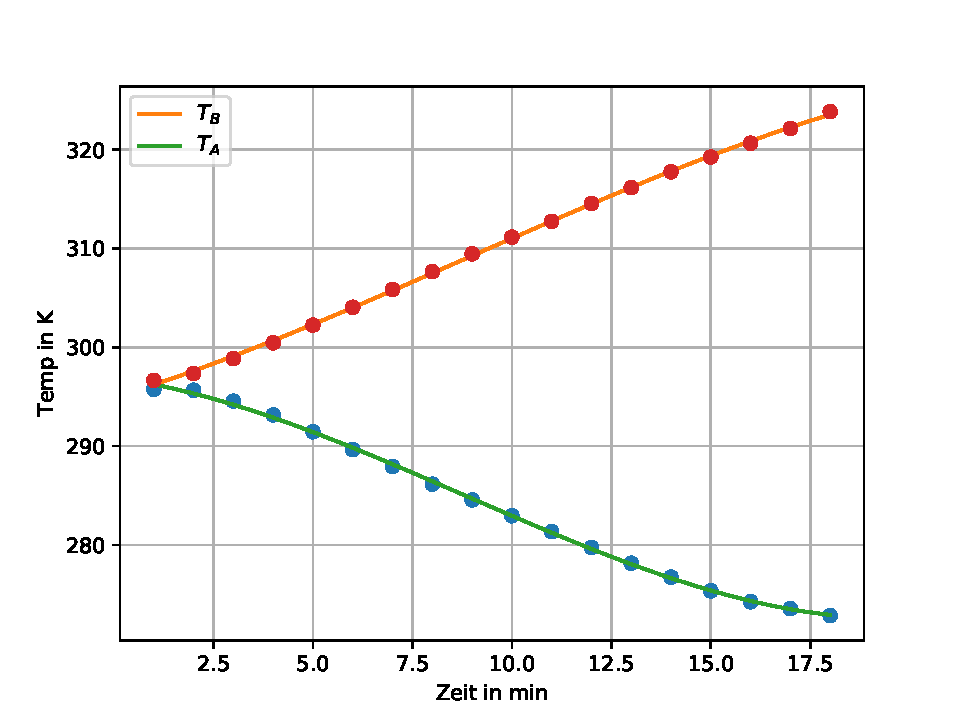
\includegraphics[width=\textwidth]{plot.pdf}
%  \caption{Messung}
%  \label{Messung}
%\end{figure}
%
%\newpage


\nocite{*}
\printbibliography

\begin{figure}
  \centering
  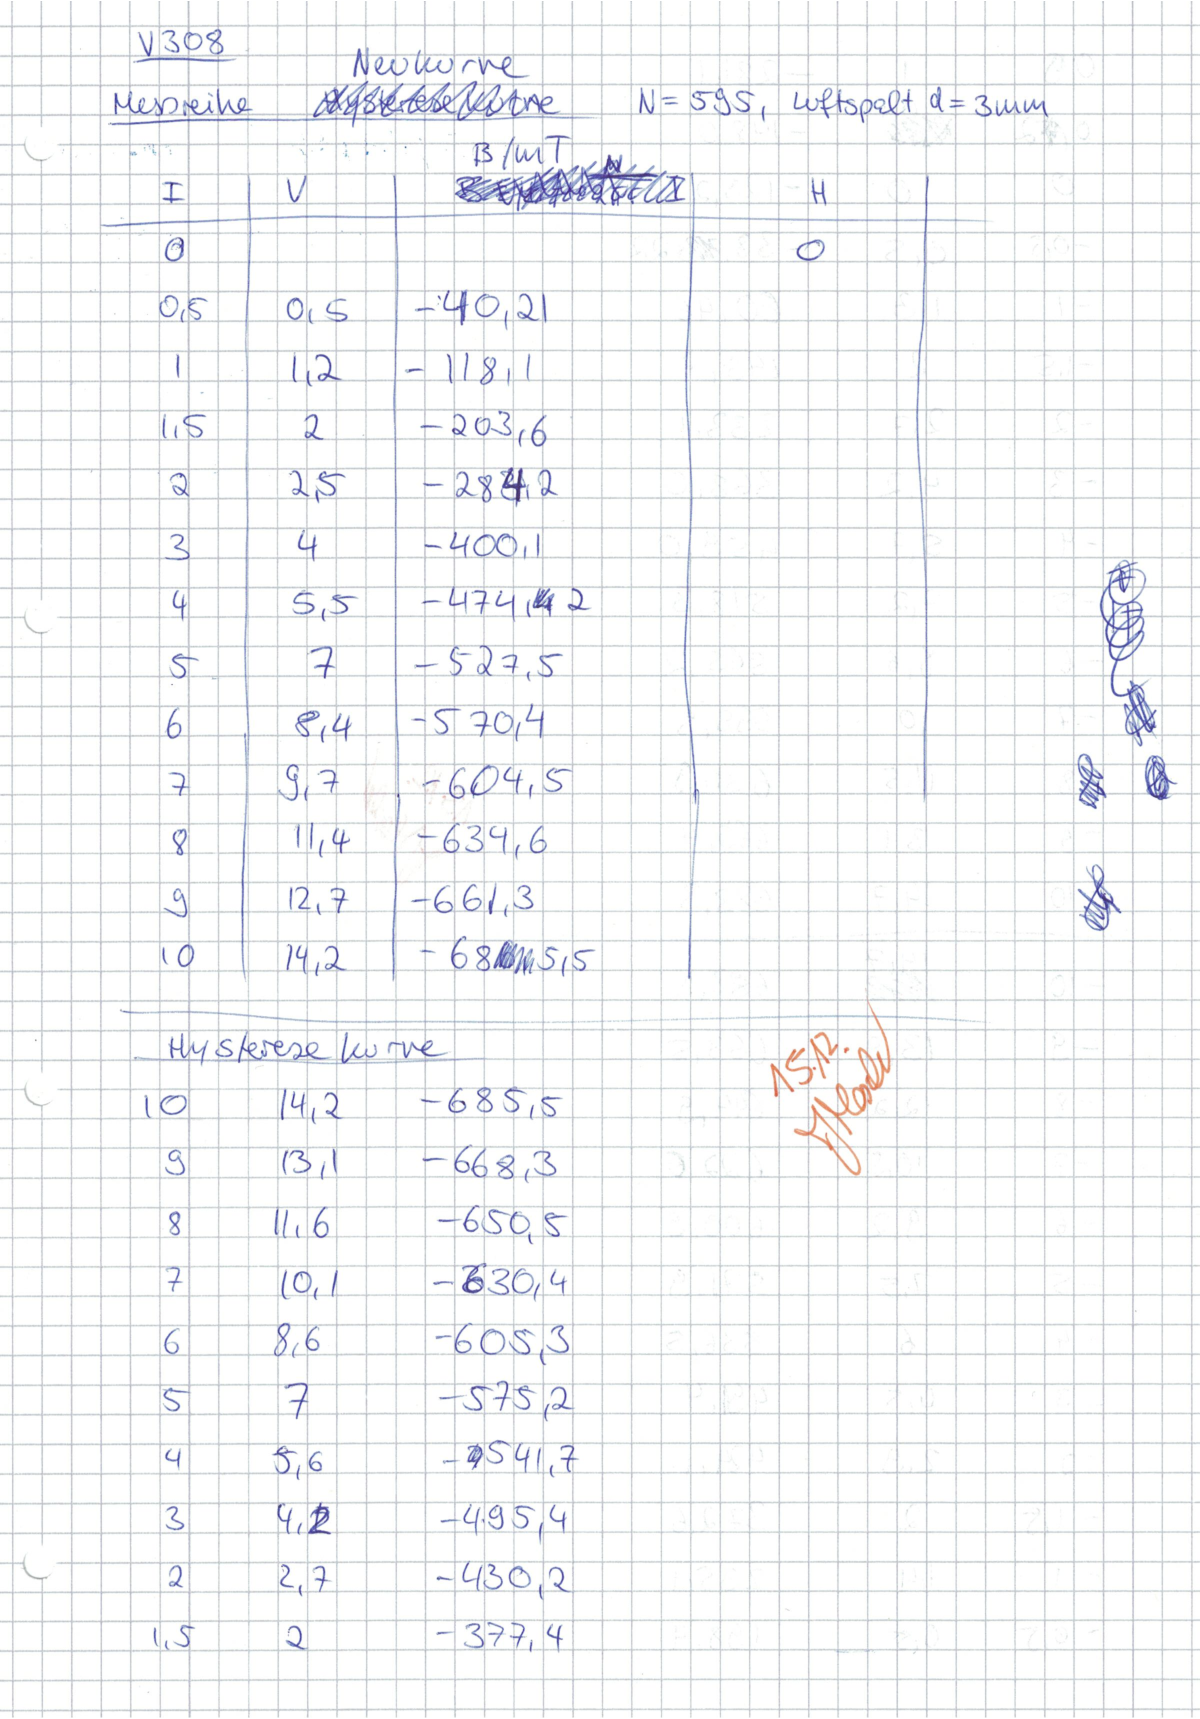
\includegraphics[width=\textwidth]{OMD1.pdf}
  \caption{Originale Messdaten}
  \label{fig:OMD1}
\end{figure}
\begin{figure}
  \centering
  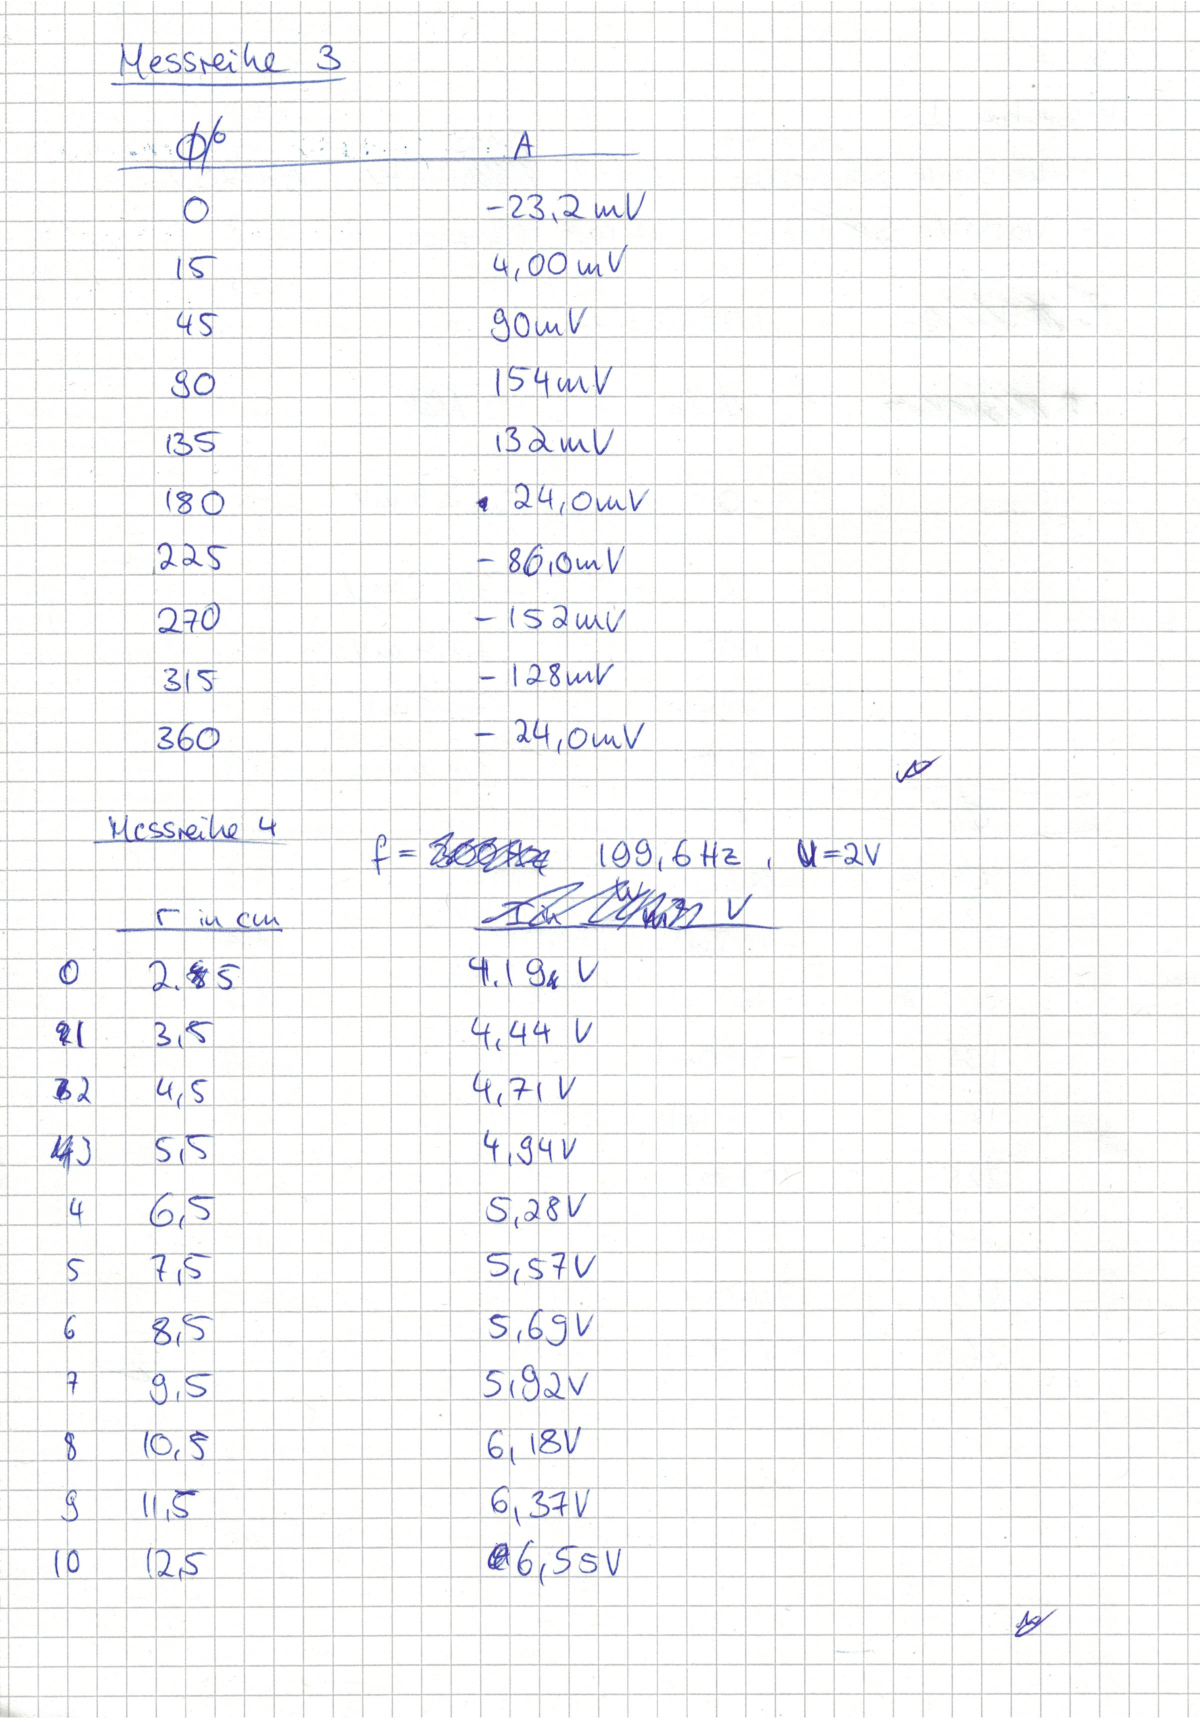
\includegraphics[width=\textwidth]{OMD2.pdf}
  \caption{Originale Messdaten}
  \label{fig:OMD2}
\end{figure}
\begin{figure}
  \centering
  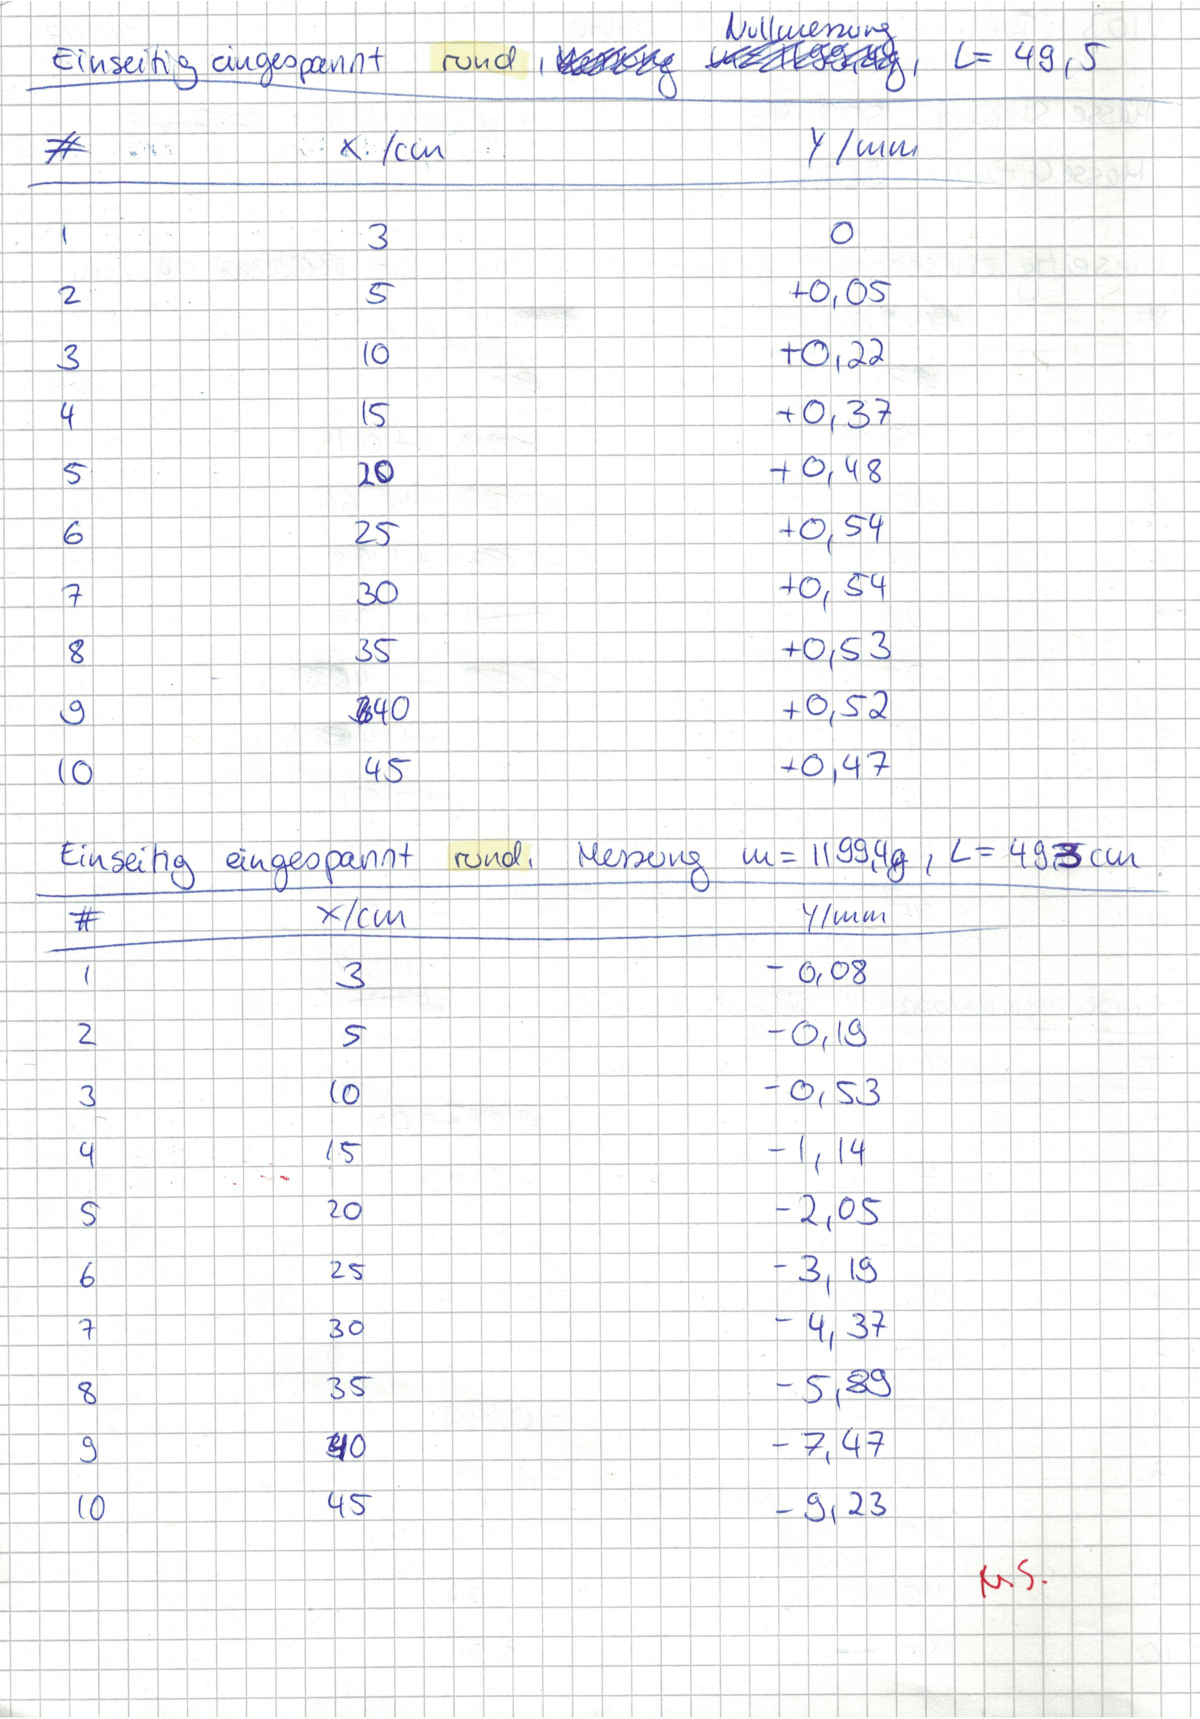
\includegraphics[width=\textwidth]{OMD3.pdf}
  \caption{Originale Messdaten}
  \label{fig:OMD3}
\end{figure}

\end{document}
